% Conceptual figure C3 -- stock behavior versus one bounded stealing pass.
% Owner: narrative writer. Vector standalone TikZ; compiled to c3_stock_vs_steal.pdf
% and included by paper/03-background-motivations.tex (figure*, double column).
% amber = encrypted/pending, teal = decrypted/ready, blue = the stealing action,
% dark = ordering barrier. Semantics reinforced by labels, numbers, line styles.
\documentclass[border=3pt]{standalone}
\usepackage{tikz}
\usepackage[T1]{fontenc}
\usetikzlibrary{arrows.meta,positioning,fit,backgrounds}

\definecolor{cAmber}{HTML}{E69F00}
\definecolor{cTeal}{HTML}{009E73}
\definecolor{cBlue}{HTML}{0072B2}
\definecolor{cInk}{HTML}{222222}

\begin{document}
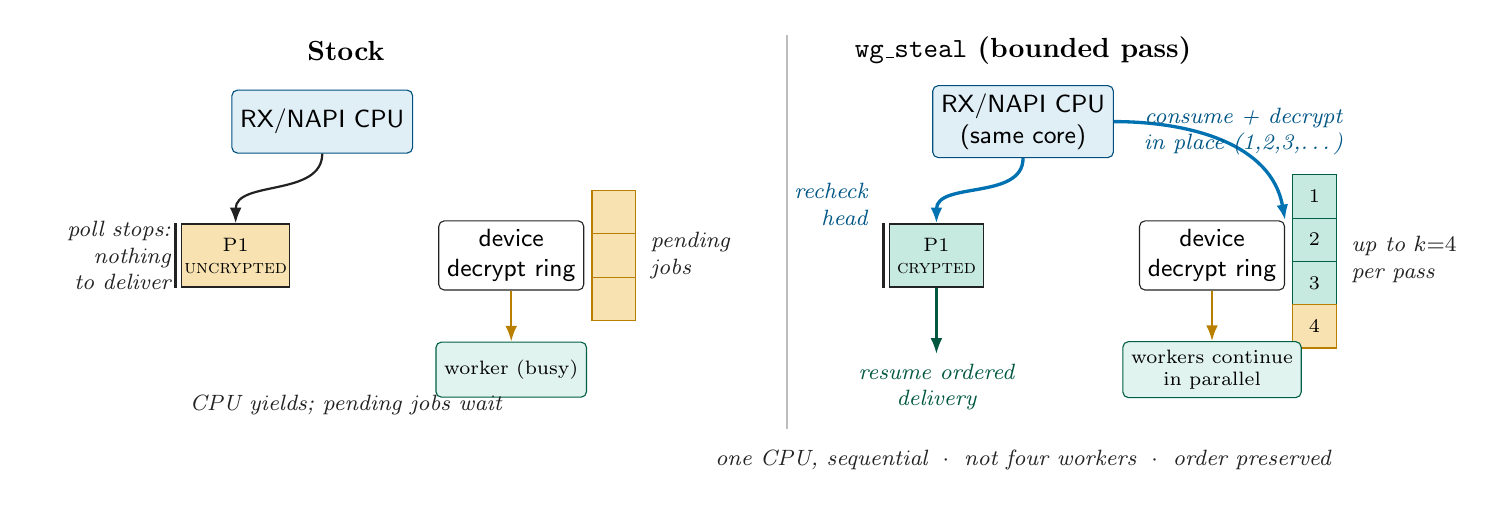
\begin{tikzpicture}[
  font=\sffamily\small,
  >={Latex[length=2mm]},
  cpu/.style={draw=cBlue!70!black,fill=cBlue!12,rounded corners=2pt,align=center,minimum height=8mm,inner sep=3pt},
  ring/.style={draw=cInk,rounded corners=2pt,align=center,minimum height=8mm,inner sep=3pt},
  job/.style={draw=cAmber!80!black,fill=cAmber!30,minimum width=5.5mm,minimum height=5.5mm,inner sep=0pt,font=\scriptsize},
  jobd/.style={draw=cTeal!60!black,fill=cTeal!22,minimum width=5.5mm,minimum height=5.5mm,inner sep=0pt,font=\scriptsize},
  head/.style={draw=cInk,minimum width=12mm,minimum height=8mm,align=center,inner sep=1pt,font=\scriptsize},
  wk/.style={draw=cTeal!60!black,fill=cTeal!12,rounded corners=2pt,align=center,font=\scriptsize,minimum height=7mm,inner sep=3pt},
  flow/.style={->,thick,cInk},
  steal/.style={->,very thick,cBlue},
  note/.style={font=\footnotesize\itshape,text=cInk},
  panel/.style={draw=cInk!35,rounded corners=3pt,dashed}
]

% =================== Panel A: Stock ===================
\begin{scope}[local bounding box=A]
  \node[cpu] (cpuA) at (2.0,0) {RX/NAPI CPU};
  \node[head,fill=cAmber!30] (headA) at (0.9,-1.7)
       {P1\\\textsc{uncrypted}};
  \draw[cInk,line width=1pt] ([xshift=-2pt]headA.north west) -- ([xshift=-2pt]headA.south west);
  \node[ring] (ringA) at (4.4,-1.7) {device\\decrypt ring};
  \node[job] (a1) at (5.7,-1.15) {};
  \node[job] (a2) at (5.7,-1.7) {};
  \node[job] (a3) at (5.7,-2.25) {};
  \node[note,anchor=west,align=left] at (6.05,-1.7) {pending\\jobs};

  % poll reaches head and stops
  \draw[flow] (cpuA.south) to[out=-90,in=90] (headA.north);
  \node[note,anchor=east,align=right,text width=17mm] at (0.2,-1.7) {poll stops:\\nothing to deliver};

  \node[wk] (wkA) at (4.4,-3.15) {worker (busy)};
  \draw[flow,cAmber!80!black] (ringA.south) -- (wkA.north);
  \node[note,anchor=north,align=center] at (2.3,-3.35) {CPU yields; pending jobs wait};
\end{scope}
\node[font=\bfseries] at (2.3,0.9) {Stock};

% divider
\draw[cInk!30,thick] (7.9,1.1) -- (7.9,-3.9);

% =================== Panel B: wg_steal ===================
\begin{scope}[local bounding box=B,shift={(8.7,0)}]
  \node[cpu] (cpuB) at (2.2,0) {RX/NAPI CPU\\(same core)};
  \node[ring] (ringB) at (4.6,-1.7) {device\\decrypt ring};
  % four jobs, first three already stolen+decrypted (teal, numbered), one pending
  \node[jobd] (b1) at (5.9,-0.95) {1};
  \node[jobd] (b2) at (5.9,-1.5) {2};
  \node[jobd] (b3) at (5.9,-2.05) {3};
  \node[job]  (b4) at (5.9,-2.6) {4};
  \node[note,anchor=west,align=left] at (6.25,-1.75) {up to $k{=}4$\\per pass};

  % the same CPU consumes + decrypts jobs sequentially (blue)
  \draw[steal] (cpuB.east) to[out=0,in=100] (ringB.north east);
  \node[note,text=cBlue!75!black,anchor=south,align=center] at (5.0,-0.55)
       {consume + decrypt\\in place (1,2,3,\dots)};

  % head becomes ready, resume delivery
  \node[head,fill=cTeal!22] (headB) at (1.1,-1.7) {P1\\\textsc{crypted}};
  \draw[cInk,line width=1pt] ([xshift=-2pt]headB.north west) -- ([xshift=-2pt]headB.south west);
  \draw[steal] (cpuB.south) to[out=-90,in=90] (headB.north);
  \node[note,anchor=east,align=right,text width=16mm,text=cBlue!75!black] at (0.35,-1.05) {recheck head};
  \draw[flow,cTeal!55!black] (headB.south) to[out=-90,in=90] (1.1,-2.95);
  \node[note,text=cTeal!55!black,anchor=north,align=center] at (1.1,-2.95) {resume ordered\\delivery};

  % workers keep running in parallel
  \node[wk] (wkB) at (4.6,-3.15) {workers continue\\in parallel};
  \draw[flow,cAmber!80!black] (ringB.south) -- (wkB.north);
\end{scope}
\node[font=\bfseries] at (10.9,0.9) {\texttt{wg\_steal} (bounded pass)};

% shared caption cues (kept minimal; full text in the LaTeX caption)
\node[note,anchor=north,align=center] at (10.9,-4.05)
     {one CPU, sequential $\;\cdot\;$ not four workers $\;\cdot\;$ order preserved};

\end{tikzpicture}
\end{document}
